\chapter{AWS am Beispiel einer Sharing Energy Plattform}\label{chapter:kapitellabel} %%%%%%%%%%%%%%%%%%%%%%%%%%%%
Nachfolgend möchte ich anhand eines Beispiels aus dem Energiemarkt einige Dienste von AWS näher betrachten und ihre Wirkungsweise im Zusammenhang darstellen.

\section{Das Fallbeispiel}
\label{sec:fallbeispiel}
\\ Bei LichtBlick, Deutschlands größtem unabhängigen Ökostromanbieter, arbeitet aktuell ein Team an einer neuen Plattform-Idee. Grundsätzlich soll es möglich sein, dass sich Personen gegenseitig ihren selbst erzeugten Ökostrom verkaufen, ohne dass ein Stromhändler dazwischen hängt. Ähnliche Produkte gibt es bereits auf dem niederländischen und dem australischen Markt, jedoch noch nicht in Deutschland. Grund hierfür sind diverse Regularien, die es Besitzern von Wind-, Wasserkraft-, Photovoltaik- und Kraft-Wärme-Kopplungs-Anlagen erschweren, ihren Strom direkt zum Verkauf an andere Personen anzubieten. Da die Entwicklung in diesem Bereich noch recht unklar ist, dennoch erste Ideen auf dem deutschen Markt vertestet werden wollen, entscheidet sich das Team für eine agile und schlanke Herangehensweise. Daher fiel die Wahl bei der Frage nach der erforderlichen IT-Infrastruktur auf Amazon Web Services.


\section{IT-Infrastruktur}
\label{sec:infrastruktur}

TODO Schaubild

\section{Virtuelle Server}

\cite{aws:general}

\section{Das Zusammenspiel der Dienste}
\label{sec:spiel}
Beispiel Cloud Comp Kap 4.1.7

\begin{figure}[!ht]
  \centering
  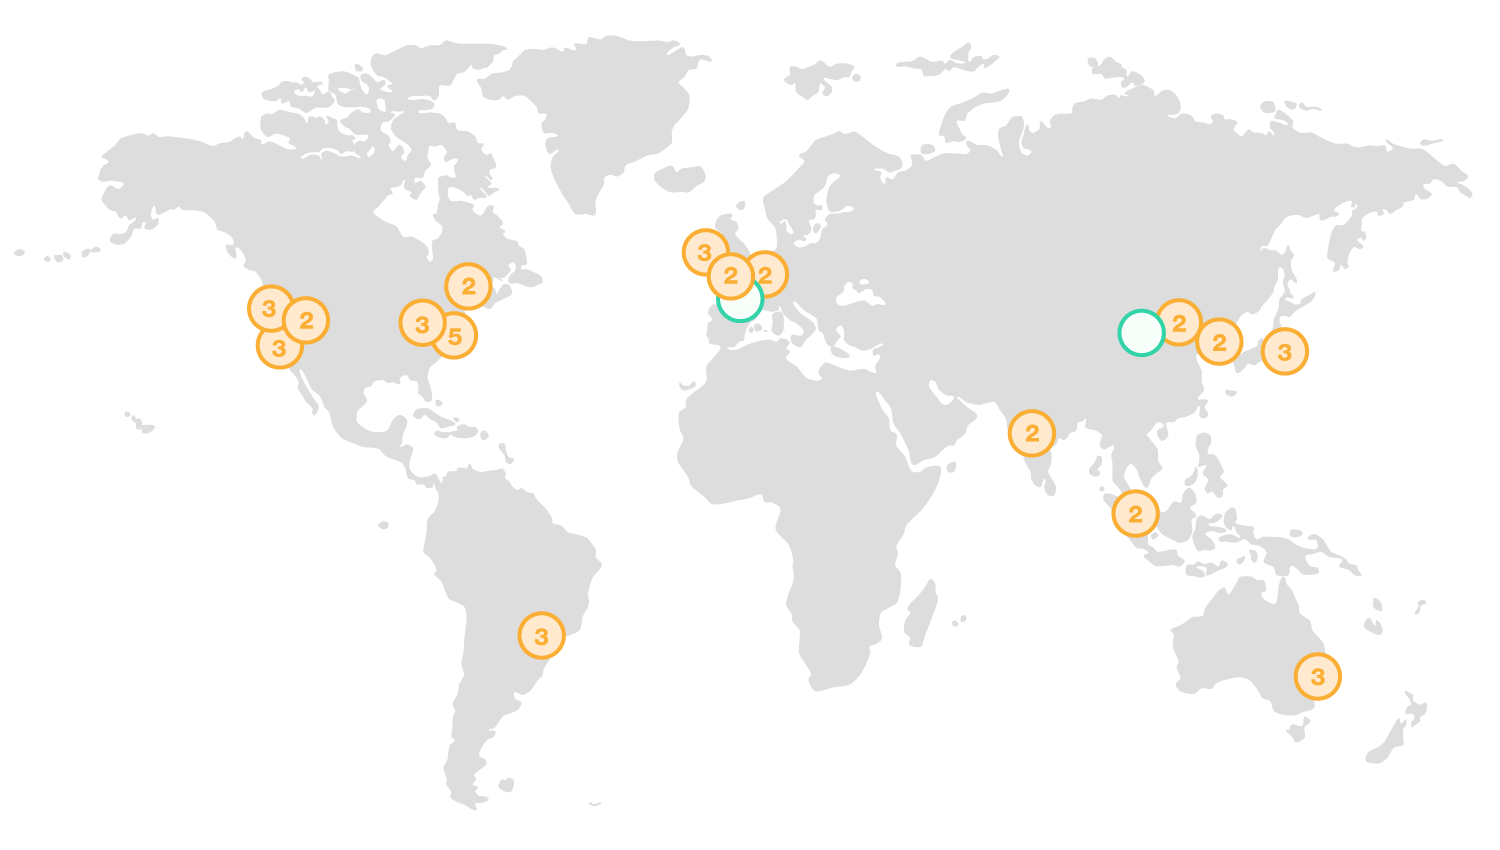
\includegraphics[width=0.9\textwidth]{images/regions.png}
  \caption{weltweite Infrastruktur (orange: Region mit x AZs, weiß/grün: geplante Region) \cite{aws:regions}}
\end{figure}


% keep an blank line above
